\documentclass[runningheads]{llncs}
%
\usepackage[T1]{fontenc}
\usepackage{graphicx}
\usepackage{amsmath,amssymb}
\usepackage{booktabs}
\usepackage{multirow}
\usepackage{array}
\usepackage{float}
%
\emergencystretch=3em
\AtBeginDocument{\renewcommand{\doi}[1]{doi:#1}}
\makeatletter
\renewcommand\section{\@startsection{section}{1}{\z@}{-12\p@ \@plus -4\p@ \@minus -2\p@}{6\p@}{\normalfont\large\bfseries\boldmath\rightskip=\z@ \@plus 8em\pretolerance=10000 }}
\renewcommand\subsection{\@startsection{subsection}{2}{\z@}{-10\p@ \@plus -3\p@ \@minus -2\p@}{4\p@}{\normalfont\normalsize\bfseries\boldmath\rightskip=\z@ \@plus 8em\pretolerance=10000 }}
\makeatother
\linespread{0.95}
\setlength{\abovedisplayskip}{4pt plus 1pt minus 2pt}\setlength{\belowdisplayskip}{4pt plus 1pt minus 2pt}\setlength{\abovedisplayshortskip}{2pt}\setlength{\belowdisplayshortskip}{2pt}
\renewcommand{\arraystretch}{0.94}
\renewcommand{\topfraction}{0.95}\renewcommand{\textfraction}{0.05}\renewcommand{\floatpagefraction}{0.8}
\setlength{\textfloatsep}{4pt plus 2pt minus 2pt}\setlength{\abovecaptionskip}{3pt}\setlength{\belowcaptionskip}{0pt}\setlength{\floatsep}{4pt plus 2pt minus 2pt}\setlength{\intextsep}{4pt plus 2pt minus 2pt}
\begin{document}
%
\title{GIS-Based Smart Village Infrastructure Planning Using DINOv2 Segmentation, Graph-Based Connectivity Analysis, and A$^{*}$ Route Planning}
%
\titlerunning{GIS-Based Smart Village Infrastructure Planning}
%
\author{Ramakrishna Kolikipogu\and Pendyala Archana\and Palamakula Swathi}
%
\authorrunning{R. Kolikipogu et al.}
%
\institute{Department of Information Technology, Chaitanya Bharathi Institute of Technology (A), Hyderabad, India\\
\email{krkrishna.cse@gmail.com}\\
\email{pendyalaarchanareddy98@gmail.com}\\
\email{swathip\_it@cbit.ac.in}}
%
\maketitle
%
\begin{abstract}
Rural infrastructure planning matters for living standards, but field-survey approaches are slow and hard to scale. This paper presents StrongDINOv2Seg, coupling a DINOv2 vision-transformer encoder with an FPN, Atrous Spatial Pyramid Pooling (ASPP), and a residual decoder to segment LoveDA imagery into its seven semantic classes (Background, Building, Road, Water, Barren, Forest, Agriculture; the no-data index is ignored). Trained for 10 epochs on combined Rural/Urban LoveDA, the model reaches a best validation mIoU of 53.80\% and mDice of 68.91\% at epoch 4 (no test-set evaluation was performed). An OpenCV/NetworkX/SciPy stage then performs building detection, road skeletonization, graph construction, KD-tree connectivity, and A$^{*}$ route planning over a land-cover-weighted cost surface, generating raster-based computational connectivity proposals for isolated buildings. On a representative tile with 14 buildings, connectivity rises from 28.57\% to 100\% via 10 proposed segments (2,029.94 px total, path efficiency 0.86); over ten further tiles (54 buildings), connectivity rises from 40.74\% to 96.30\% via 30 connections (efficiency 0.931). All figures are validation-split results with no held-out test set; planning covers only the selected LoveDA tiles; and route outputs are decision-support proposals, not field-validated and not establishing engineering, terrain, environmental, cost, legal, or social feasibility.
\keywords{DINOv2 \and Semantic segmentation \and ASPP \and FPN \and LoveDA dataset \and Smart village \and Rural infrastructure planning \and Road extraction \and Building detection \and Connectivity analysis \and KD-tree \and A$^{*}$ path planning \and OpenCV}
\end{abstract}


%
\section{Introduction}
Characterising rural infrastructure -- roads, buildings, water, agricultural land -- matters for living standards~\cite{hinton1996}. Poor road connectivity is a recognised barrier to healthcare access~\cite{verma2020}, and infrastructural gap analysis has been used to prioritise rural investment~\cite{kapoor2021}. GIS-based imagery analysis supports this, but manual survey is slow and hard to scale; benchmarks such as SpaceNet~\cite{vanetten2018} and DeepGlobe~\cite{demir2018} have driven progress in automated extraction, motivating its combination with planning.

This paper describes StrongDINOv2Seg: a DINOv2-based segmentation model paired with a downstream pipeline -- road extraction, skeletonization, graph construction, KD-tree connectivity, and A$^{*}$ route planning -- that turns segmentation into raster-based computational connectivity proposals. It is evaluated on LoveDA segmentation quality, a representative planning tile, and a ten-tile sample, reporting class-wise metrics, an A$^{*}$ cost formulation, and a radius-sensitivity analysis.

\section{Related Work}
\textbf{Segmentation.} SegFormer~\cite{xie2021} and UNetFormer~\cite{wang2022unet} (on LoveDA) advanced transformer segmentation but need large labelled sets; DINOv2~\cite{oquab2023} is self-supervised but not built for dense satellite classification, addressed here via fine-tuning with an ASPP/FPN decoder. \textbf{Road/building extraction.} D-LinkNet~\cite{zhou2018} won the DeepGlobe road-extraction challenge; attention, atrous/strip, fusion, and dual-decoder extractors followed~\cite{bai2025,ma2026,zhang2024,qu2025}, with several targeting road topology~\cite{kamada2021,mattyus2017,xu2023,liu2017}. Ayala et al.~\cite{ayala2021} jointly detected buildings and roads from Sentinel imagery, mirroring our two-class task; VHR building/settlement classification~\cite{dimassi2024,kakooei2026}, a modified ViT for rural land cover~\cite{wassan2025}, and MAP-Net~\cite{zhu2021} for small buildings are also relevant. \textbf{GIS planning and routing.} OSMnx~\cite{boeing2017} popularised the NetworkX street-graph used in our connectivity stage; Verma and Dash~\cite{verma2020} modelled rural healthcare accessibility via GIS network analysis, and Kapoor et al.~\cite{kapoor2021} ranked Telangana village infrastructure gaps, both relevant to prioritising isolated buildings. Wang et al.~\cite{wang2022astar} proposed weighted, cost-aware A$^{*}$ routing, related to our traversal-cost surface. These works generally treat segmentation, extraction, or GIS accessibility in isolation.

\textbf{Problem and contributions.} A pipeline that only classifies land cover does not, by itself, tell a planner where new access roads are needed. Planning requires a rural land-cover segmenter, a discrete inventory of buildings and roads, and a rule for deciding which buildings need access and where; prior systems address these separately. This paper integrates them as an engineering decision-support demonstration whose outputs are raster-based computational connectivity proposals, not field-validated engineering plans. The main contributions are: (i) integrating a DINOv2-based segmentation model with an explicit cost-weighted A$^{*}$ route-planning stage; (ii) class-wise and aggregate segmentation metrics; (iii) an explicit A$^{*}$ traversal-cost surface; (iv) evaluation on a representative tile, a radius-sensitivity sweep, and a pooled ten-tile sample; and (v) explicit limitations. No component is individually novel; the contribution is their integration.

\section{Proposed Methodology}
\subsection{Overall System Architecture}
The pipeline has two stages: StrongDINOv2Seg classifies each pixel into one of eight indices per the official LoveDA encoding (0 = no-data, ignored; 1--7 = Background, Building, Road, Water, Barren, Forest, Agriculture); a second stage then uses classical vision and graph algorithms to detect buildings, skeletonize roads, mark existing connections, and plan segments for isolated ones (Sect.~\ref{sec:setup}).

\subsection{DINOv2 Encoder, FPN, ASPP, and Decoder}
A pretrained \texttt{facebook/dinov2-base} Vision Transformer with patch size 14 serves as the fine-tuned encoder. Inputs are resized to $560\times560$ and embedded into $40\times40$ patch tokens. Hidden states are taken from layers 3, 6, 9, and 12 (768-dimensional each):
\begin{equation}
z'_l=\mathrm{MSA}(\mathrm{LN}(z_{l-1}))+z_{l-1},\qquad z_l=\mathrm{MLP}(\mathrm{LN}(z'_l))+z'_l
\end{equation}
where MSA is multi-head self-attention, LN is layer normalisation, and MLP is the feed-forward block. Each $40\times40\times768$ feature map is projected to 256 channels ($P_l=\mathrm{Conv}_{1\times1}(f_l)$), concatenated, and fused:
\begin{equation}
F_{\mathrm{fuse}}=\mathrm{Conv}_{1\times1}\big(\mathrm{Concat}(P_3,P_6,P_9,P_{12})\big)
\end{equation}
ASPP is applied with dilation rates 6, 12, 18, a $1\times1$ branch, and a global-pooling branch, giving a 256-channel output: $\mathrm{ASPP}(x)=\mathrm{Proj}(\mathrm{Concat}(B_1,\dots,B_5))$. A residual decoder ($R(x)=F(x)+x$) restores spatial resolution through four $2\times$ upsampling stages ($256\to256\to128\to64\to32$ channels), producing a $640\times640$ map resized to $560\times560$, followed by a final $1\times1$ convolution to eight classes.

\subsection{Loss Function}
Training uses a composite loss:
\begin{equation}
L_{\mathrm{total}}=0.5\,L_{\mathrm{CE}}+0.4\,L_{\mathrm{Dice}}+0.1\,L_{\mathrm{boundary}},\qquad L_{\mathrm{Dice}}=1-\frac{2|P\cap G|+\epsilon}{|P|+|G|+\epsilon}
\end{equation}
where $L_{\mathrm{CE}}$ is pixel-wise cross-entropy and $L_{\mathrm{boundary}}$ is a Sobel-edge-weighted boundary term; both CE and Dice ignore the no-data index (0). An auxiliary deep-supervision loss weight is defined but inactive, since the decoder exposes no auxiliary heads.

\section{System Architecture: Connectivity Analysis and Route Planning}
\subsection{Building/Road Extraction and Connectivity Graph}
Buildings are detected via 8-connected component analysis of the Building mask (OpenCV \texttt{connectedComponentsWithStats}), discarding components under 20 px. Road pixels are cleaned by $3\times3$ closing then opening and skeletonized (scikit-image) to a one-pixel centreline, converted to an undirected NetworkX graph -- the OSMnx~\cite{boeing2017} street-graph representation -- with 8-connected edges weighted 1.0 (orthogonal) or $\sqrt2$ (diagonal). A building counts as connected if the road mask, dilated by radius $r$ (default 5 px), overlaps its expanded bounding box; for isolated buildings a KD-tree over skeleton pixels returns the nearest road pixel, or none if the skeleton is empty.

\subsection{Cost-Weighted A$^{*}$ Route Planning}
For every isolated building with a valid KD-tree target, A$^{*}$ search plans a route over an 8-connected grid, following the weighted-cost formulation adopted in GIS route-planning studies such as~\cite{wang2022astar}. Let $I(p)$ denote the predicted class index at pixel $p$:
\begin{equation}
\mathrm{cost}(p)=\begin{cases}
\infty & I(p)\in\{0,4\}\ \text{(no-data, water)}\\
1 & I(p)=3\ \text{(road)}\\
2 & I(p)=7\ \text{(agriculture)}\\
3 & I(p)=1\ \text{(background)}\\
4 & I(p)=5\ \text{(barren)}\\
5 & I(p)=2\ \text{(building)}\\
8 & I(p)=6\ \text{(forest)}
\end{cases}
\end{equation}
The search minimises $F(n)=g(n)+h(n)$ with $g$ the accumulated cost and $h$ the Euclidean heuristic; since all finite costs are $\ge1$, $h$ never overestimates, so a returned route is minimum-cost under this raster model, not a globally optimal real-world design. If A$^{*}$ fails, a straight Bresenham fallback is used; it ignores the cost surface and may cross infinite-cost pixels (e.g., water), so fallback routes are topological placeholders requiring manual re-routing, not traversable proposals. Lengths are reported in pixels on the $560\times560$ grid. LoveDA imagery has a native ground sampling distance of about $0.3$\,m at $1024\times1024$~\cite{wang2021loveda}, so after resizing the effective GSD is roughly 0.55\,m/px, e.g.\ the 202.99 px mean proposed length is approximately 110\,m; these conversions are approximate and unused in any reported metric. Routes remain pixel-space decision-support proposals, not field validated, and establish no engineering, terrain, environmental, cost, legal, or social feasibility.

\begin{table}[H]
\caption{Training configuration.}\label{tab:train}
\centering\footnotesize
\begin{tabular}{llll}
\toprule
Parameter & Value & Parameter & Value\\
\midrule
Encoder & DINOv2-base (p14) & Optimizer & AdamW\\
Resolution/classes & $560^2$ / 8 & Weight decay & $1\times10^{-4}$\\
Batch/epochs & 2 / 10 & Grad. clip/AMP & 1.0 / off\\
Enc./dec. LR & $5\times10^{-6}$ / $5\times10^{-5}$ & Loss (CE/Dice/bnd.) & .5/.4/.1\\
LR schedule & Cosine, $\eta_{\min}=10^{-7}$ & Parameters & 93.8M\\
\bottomrule
\end{tabular}
\end{table}



\begin{table}[H]
\caption{Per-class and overall (macro-averaged) segmentation metrics, epoch-4 model.}\label{tab:seg}
\centering\footnotesize
\begin{tabular}{lrrrr}
\toprule
Class & IoU (\%) & Precision (\%) & Recall (\%) & F1 (\%)\\
\midrule
Background & 54.00 & 62.09 & 80.57 & 70.13\\
Building & 66.77 & 78.77 & 81.43 & 80.08\\
Road & 56.44 & 82.46 & 64.14 & 72.15\\
Water & 71.91 & 84.65 & 82.69 & 83.66\\
Barren & 30.13 & 49.47 & 43.52 & 46.31\\
Forest & 39.86 & 61.51 & 53.11 & 57.00\\
Agriculture & 57.50 & 87.58 & 62.61 & 73.02\\
\midrule
Overall (macro avg.) & 53.80 (mIoU) & 72.36 & 66.87 & 68.91 (mDice)\\
\bottomrule
\end{tabular}
\end{table}

\subsection{Evaluation Metrics}
Segmentation uses pixel accuracy (non-background), precision, recall, F1, mIoU, and mDice, macro-averaged over the seven LoveDA classes (indices 1--7). Planning uses connectivity before/after planning, proposed-connection count, total/average road length, average nearest-road distance, and path efficiency (straight-line to planned-path ratio; 1 is most direct).

\section{Dataset, Preprocessing, and Experimental Setup}\label{sec:setup}
Data come from LoveDA~\cite{wang2021loveda} (Rural + Urban combined), a benchmark alongside SpaceNet~\cite{vanetten2018} and DeepGlobe~\cite{demir2018}. Images/masks are resized to $560\times560$ (nearest-neighbour for masks), scaled to $[0,1]$ without ImageNet normalisation, with random horizontal/vertical flips and $0^\circ/90^\circ/180^\circ/270^\circ$ rotations at training only. Masks follow the official LoveDA label encoding; index 0 (no-data) is excluded from loss and metrics, and the seven scored classes are Background, Building, Road, Water, Barren, Forest, and Agriculture. The Train split was used for training and the Val split for all reported metrics; epoch selection was also made on validation mIoU, so reported metrics are model-selection-biased and no held-out test set was used. The ten planning tiles (4216--4225) were taken from the unlabelled LoveDA Test/Rural directory, contributing to neither training loss nor epoch selection; carrying no ground-truth masks, their segmentation accuracy is unmeasured, so the planning results describe pipeline behaviour on unseen imagery without a segmentation-accuracy guarantee.

The pipeline is implemented in Python (PyTorch, Hugging Face transformers, OpenCV, scikit-image, NetworkX, SciPy, and Matplotlib) with \texttt{facebook/dinov2-base} as encoder. Training used an NVIDIA RTX A4000 GPU (16 GB); planning ran on an NVIDIA Tesla T4. Table~\ref{tab:train} lists the training configuration. The model trained end-to-end for 10 epochs (encoder at reduced LR), checkpointed on validation-mIoU improvement; epoch 4 (mIoU 0.5380, mDice 0.6891) was selected. Planning was demonstrated on LoveDA image 4216 at the default 5 px connectivity radius, with a separate tile used for the radius-sensitivity experiment.

\begin{figure}[H]
\centering
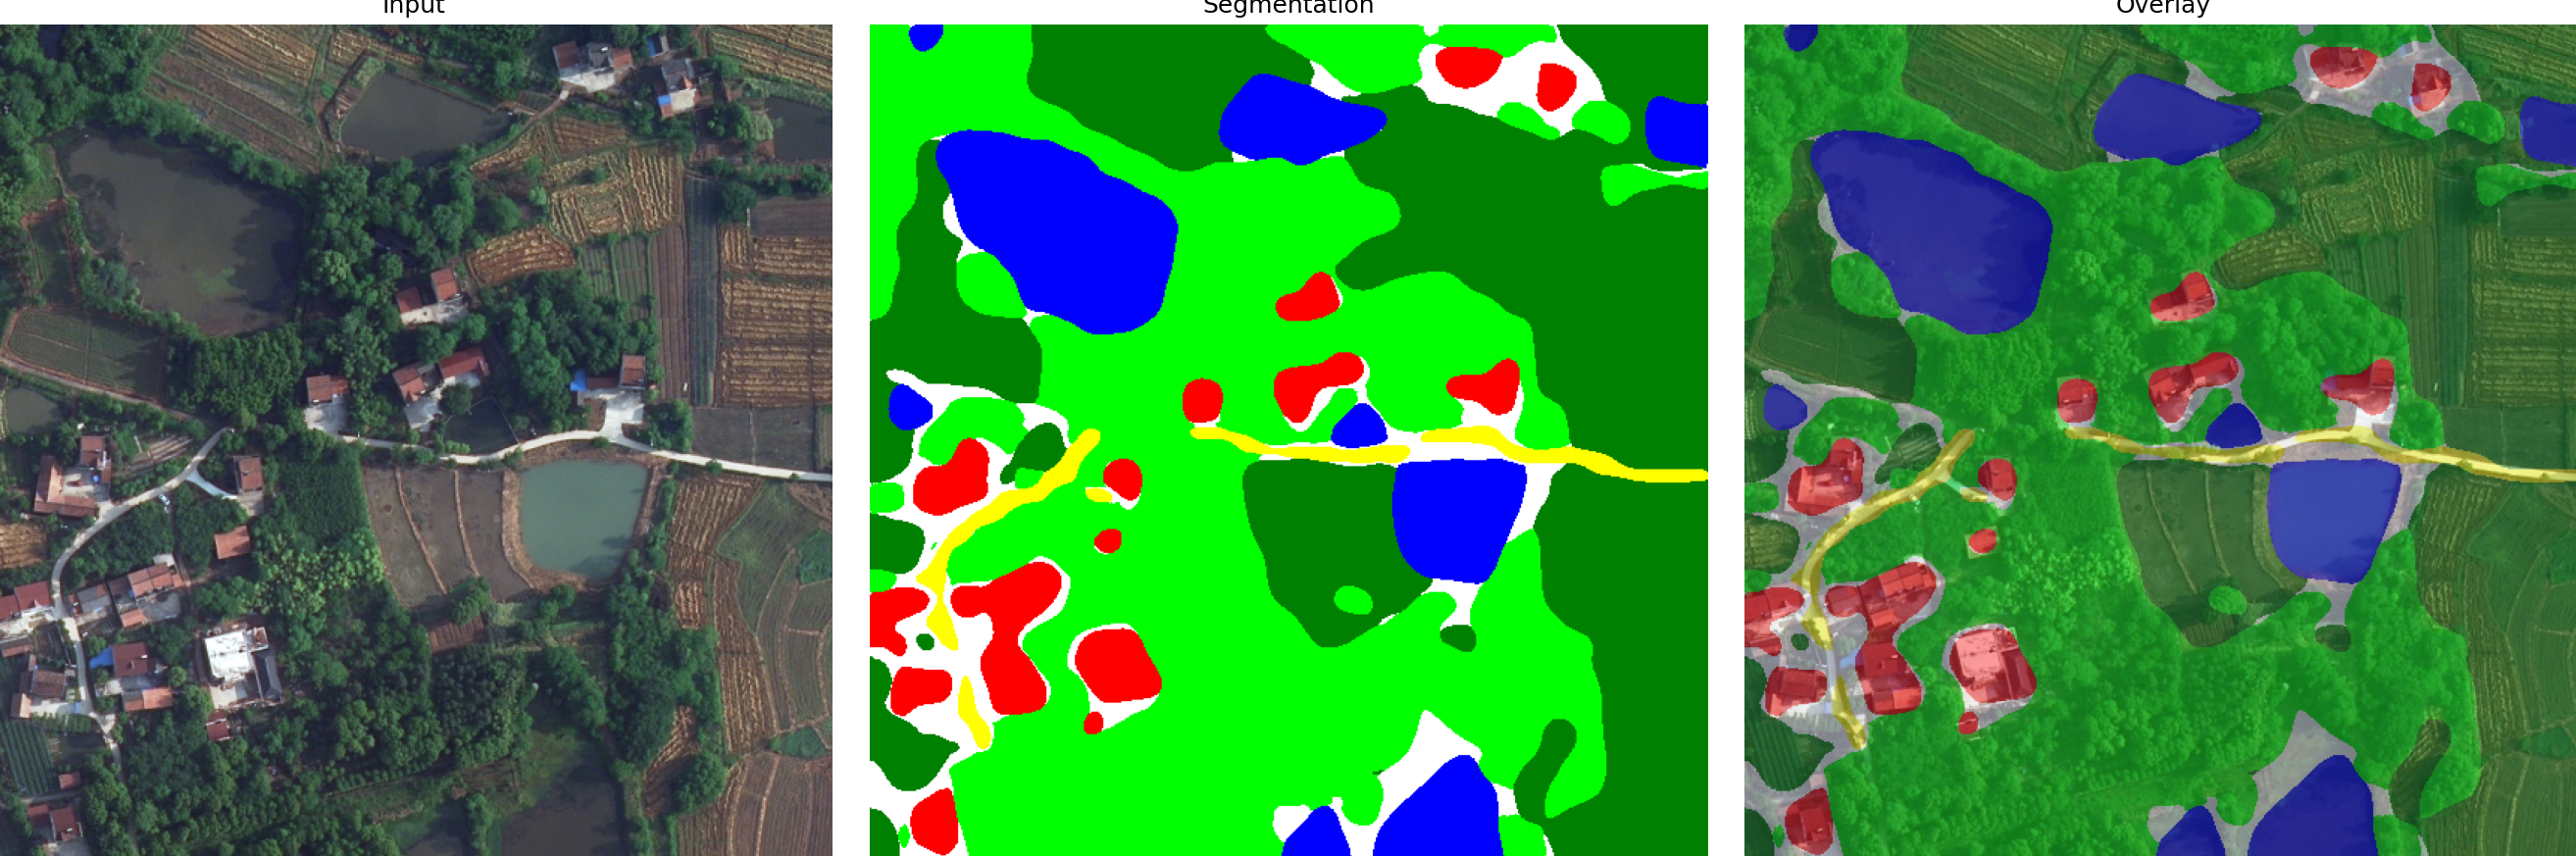
\includegraphics[width=0.75\textwidth]{figs/fig1_segmentation.png}
\caption{Segmentation output for a sample tile. Left: input image. Centre: predicted class map. Right: prediction overlaid on the input.}\label{fig:seg}
\end{figure}

\section{Results and Discussion}
\subsection{Building Detection and Segmentation Results}
On tile 4216, 8-connected component analysis of the Building mask (20-pixel minimum area) yields 14 building instances; at $r=5$ px, 4 connect to the extracted road skeleton and 10 are isolated (Fig.~\ref{fig:plan}, left) -- instance counts, distinct from the pixel-area fractions in Sect.~7.3. Table~\ref{tab:seg} reports per-class and overall metrics of the epoch-4 model (pixel accuracy 71.34\%; Fig.~\ref{fig:seg}). Accuracy peaked at 72.19\% at epoch 2, but epoch 4 was kept since mIoU was the selection criterion. Training loss fell monotonically over 10 epochs (2.0436 to 1.0488); validation mIoU rose from 0.5208 to a peak of 0.5380 at epoch 4 before plateauing (Fig.~\ref{fig:train}), motivating epoch-4 selection despite the continuing loss reduction.

\begin{figure}[H]
\centering
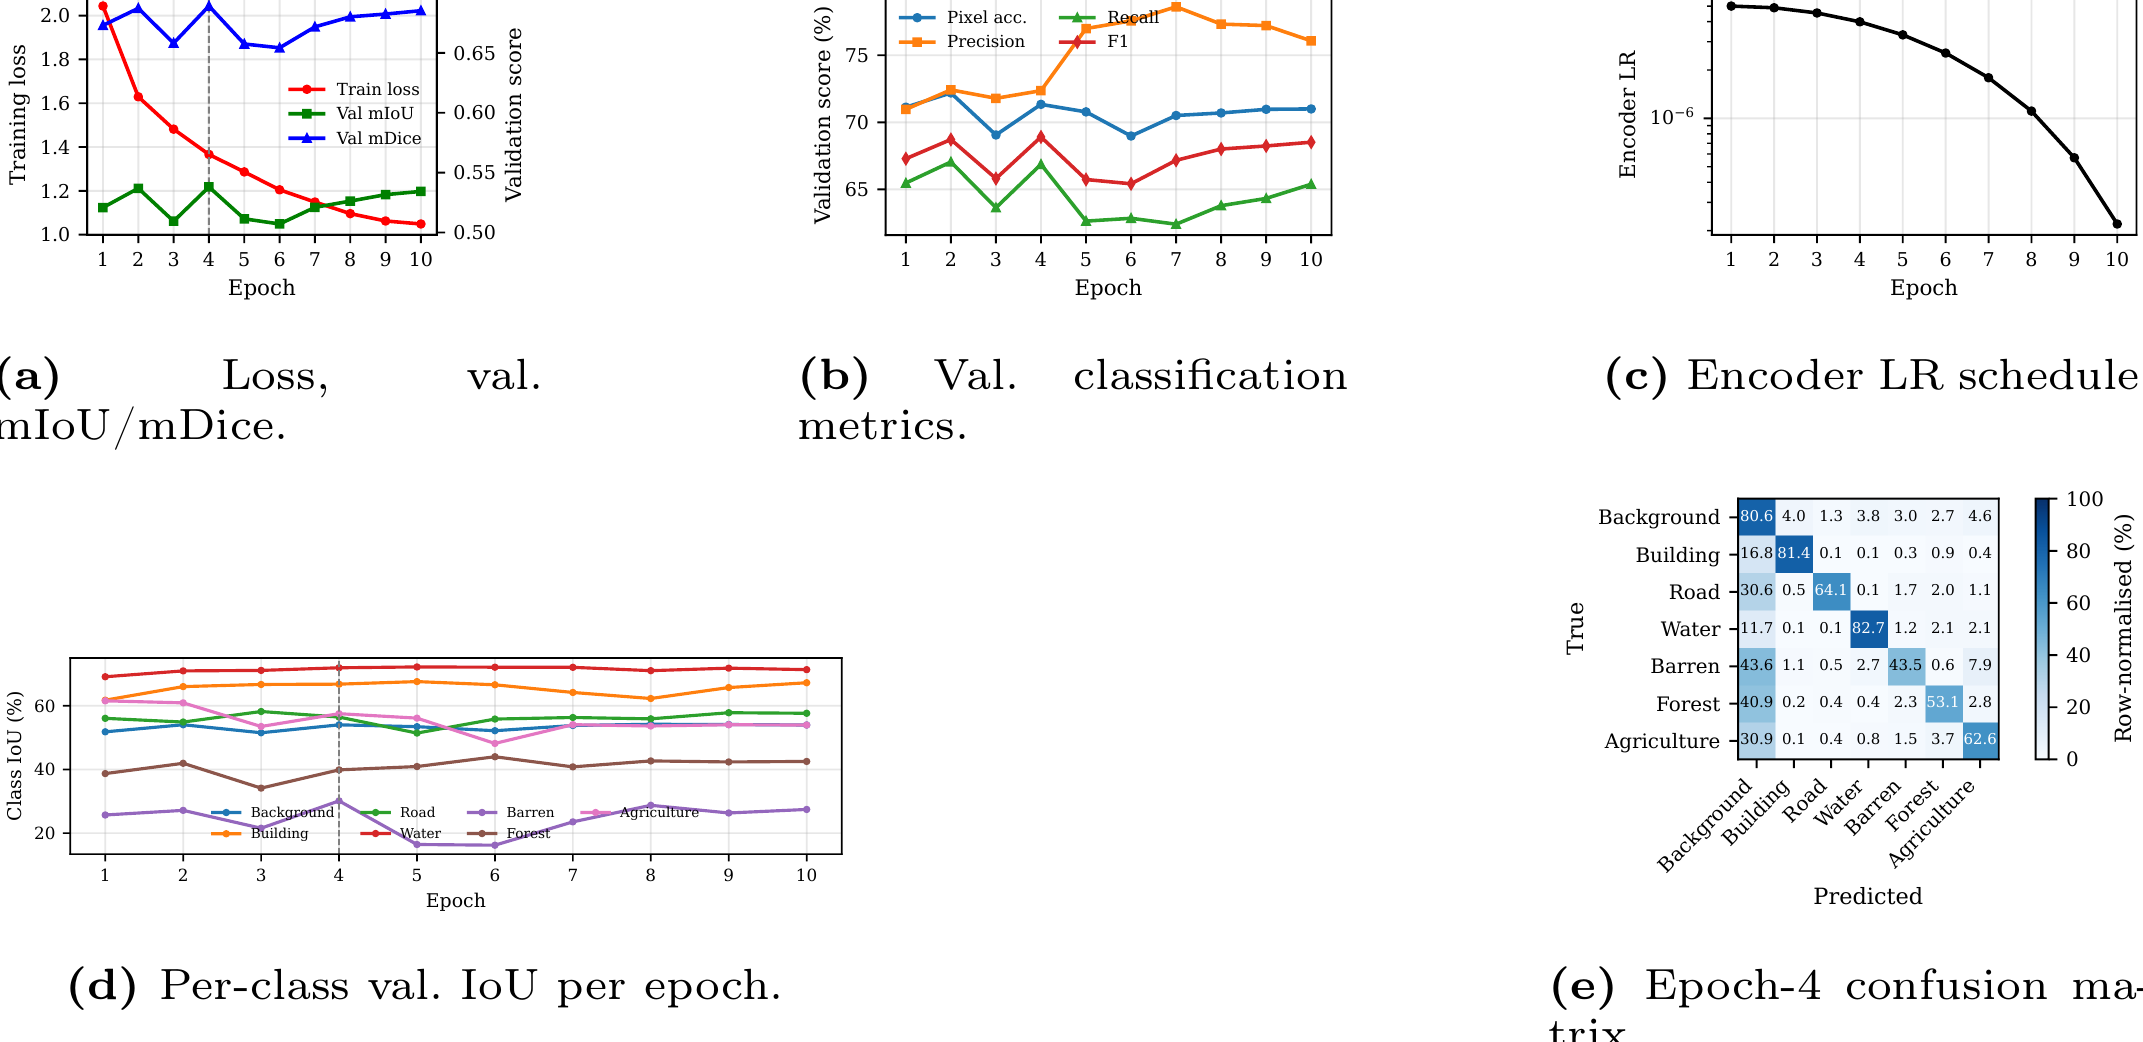
\includegraphics[width=0.85\textwidth]{figs/fig2_training.png}
\caption{Training diagnostics over ten epochs, re-plotted from the training log with official LoveDA class names. Dashed line marks epoch 4 (selected on validation mIoU); all curves are validation-split diagnostics, not held-out test results.}\label{fig:train}
\end{figure}

\subsection{Connectivity, Planning, and Sensitivity Results}
At $r=5$ px, connectivity on the representative tile (14 buildings) rose from 4 (28.57\%) to 14 (100.00\%) via 10 connections totalling 2,029.94 px (mean 202.99 px), mean nearest-road distance 170.78 px, mean path efficiency 0.86 (Fig.~\ref{fig:plan}, right). Table~\ref{tab:tile10} (left) varies $r\in\{3,5,8,10\}$ px on a different tile (15 buildings; 46.67\% connected, 8 connections at $r=5$ px, hence its differing row): a larger radius marks more buildings as already connected, so connections fall from 9 to 6 and length from 1,164.0 to 1,046.1 px, efficiency staying in 0.83--0.86.

\begin{table}[H]
\caption{Left: connectivity-radius sensitivity (separate demonstration tile). Right: aggregate ten-tile planning summary ($r=5$ px).}\label{tab:tile10}
\centering\footnotesize
\begin{minipage}[c]{0.53\textwidth}
\centering
\resizebox{\textwidth}{!}{%
\begin{tabular}{rrrrr}
\toprule
$r$ (px) & Before (\%) & After (\%) & Length (px) & Eff.\\
\midrule
3 & 40.00 & 100.0 & 1164.00 & 0.8605\\
5 & 46.67 & 100.0 & 1130.10 & 0.8502\\
8 & 53.33 & 100.0 & 1074.88 & 0.8529\\
10 & 60.00 & 100.0 & 1046.06 & 0.8307\\
\bottomrule
\end{tabular}}
\end{minipage}\hfill
\begin{minipage}[c]{0.45\textwidth}
\centering
\resizebox{\textwidth}{!}{%
\begin{tabular}{lr}
\toprule
Metric & Value\\
\midrule
Images / with proposals & 10 / 8\\
Buildings detected & 54\\
Connected before & 22 (40.74\%)\\
Connected after & 52 (96.30\%)\\
Proposed connections & 30\\
Total proposed length & 4,198.6 px\\
Mean nearest-road dist. & $162.47\pm80.88$ px\\
Mean path efficiency & $0.931\pm0.026$\\
\bottomrule
\end{tabular}}
\end{minipage}
\end{table}

\subsection{Multi-Tile and Aggregate Evaluation}
On ten LoveDA rural tiles ($r=5$ px, 20 px min.\ area), tiles 4217/4225 had no detected buildings and tiles 4219/4222 stayed at 0\% (empty skeleton, no KD-tree target) -- so 100\% post-planning connectivity is not general. Table~\ref{tab:tile10} (right): 54 buildings, connectivity 40.74\%$\to$96.30\% (+55.56 points) via 30 connections, path efficiency $0.931\pm0.026$ over 8 path-feasible tiles. Tile 4216's composition (Background 15.9\%, Building 12.9\%, Road 1.4\%, Water 3.4\%, Forest 48.5\%, Agriculture 17.9\%) matched per-class pixel counts.

\begin{figure}[H]
\centering
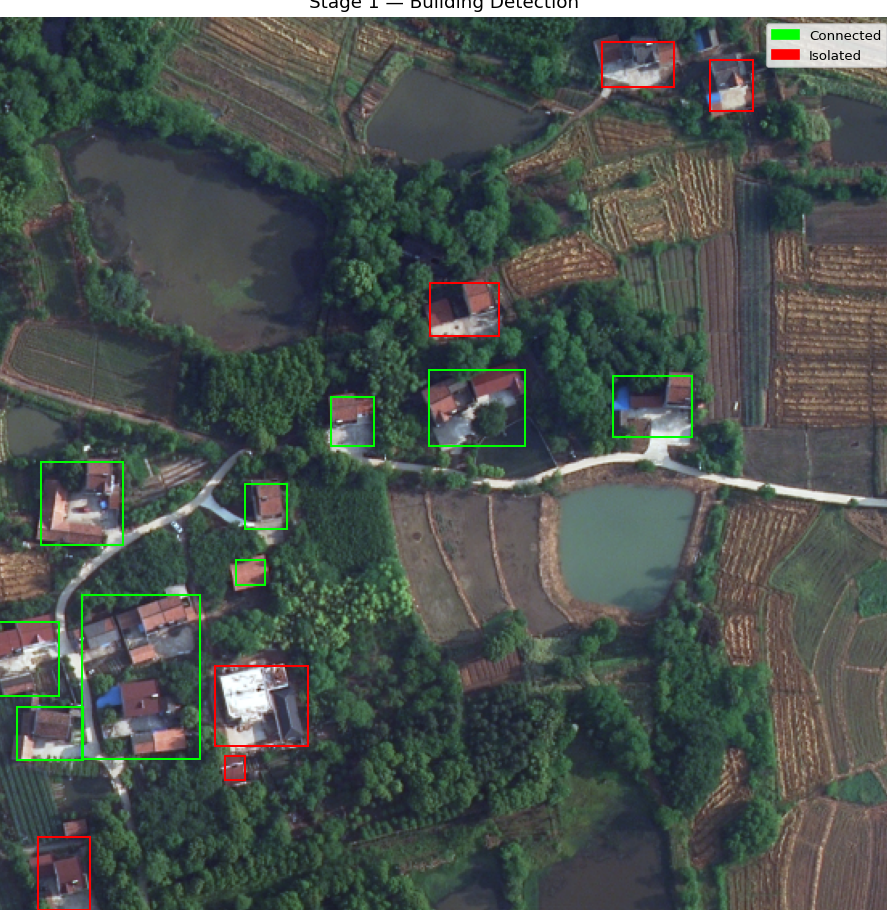
\includegraphics[width=0.43\textwidth]{figs/fig3_before.png}\hspace{0.01\textwidth}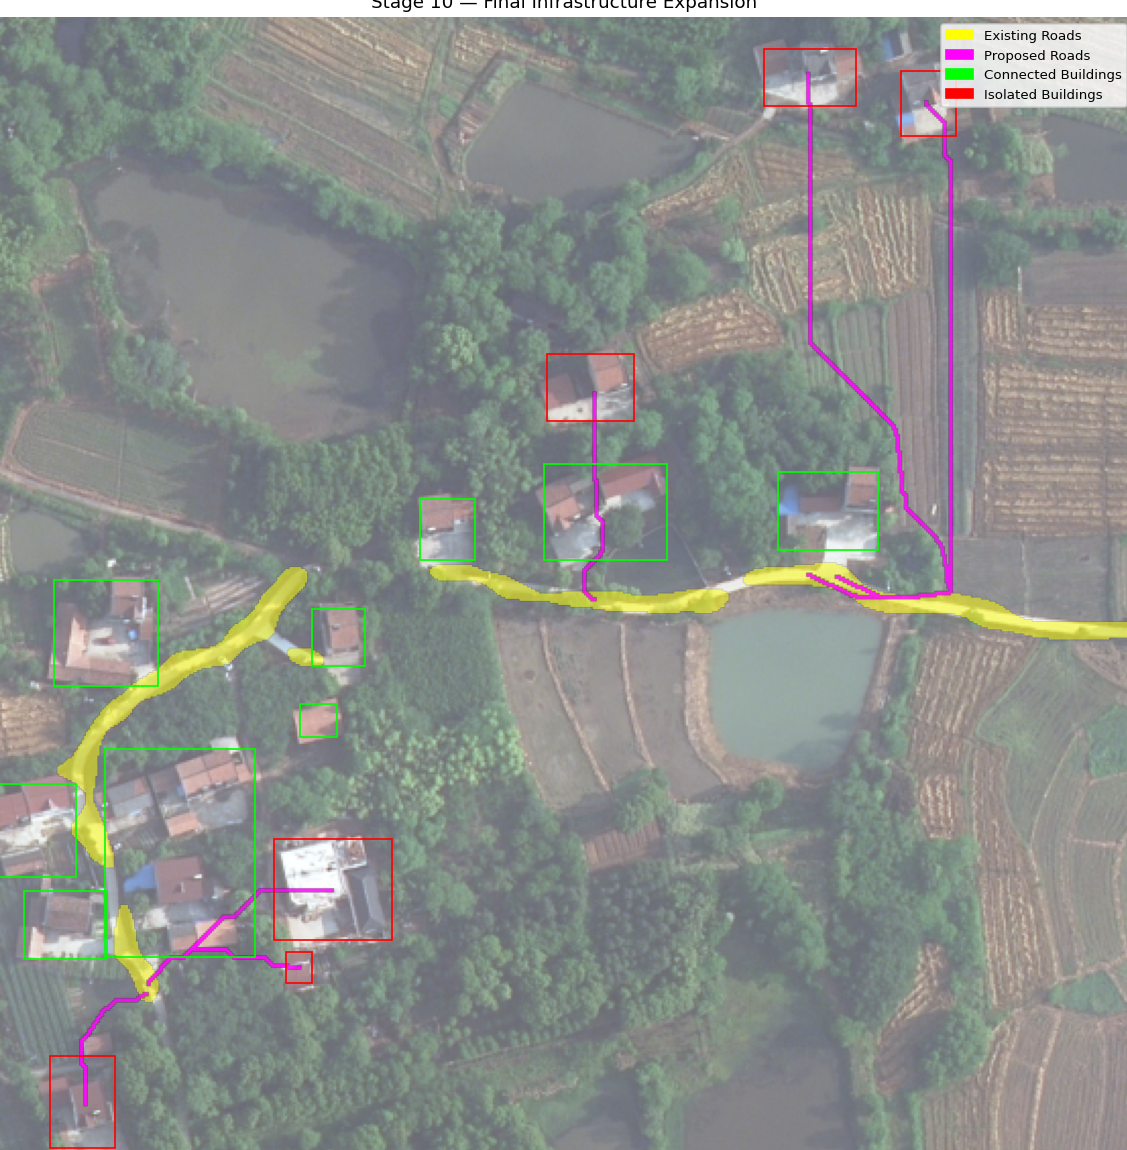
\includegraphics[width=0.43\textwidth]{figs/fig3_after.png}
\caption{Tile 4216 before (left) and after (right) planning. Green boxes: road-connected buildings (4); red: isolated (10); yellow: existing roads; magenta: A$^{*}$-planned connections.}\label{fig:plan}
\end{figure}

\subsection{Discussion}
Water scores highest on IoU/F1 (71.91\%/83.66\%), followed by Building (66.77\%/80.08\%), in line with lightweight segmenters such as UNetFormer~\cite{wang2022unet} (benchmarks differ, so no direct comparison). Background recall (80.57\%) exceeds precision (62.09\%, over-prediction); Agriculture shows the opposite (87.58\%/62.61\%, conservative); Barren and Forest remain weakest (30.13\%/39.86\% IoU); Road's 56.44\% IoU with 64.14\% recall makes broken road masks a realistic planner failure mode. Missed buildings and broken roads propagate into the component analysis, skeleton graph, and A$^{*}$ planning, so the 100\% post-planning connectivity is algorithmic, pixel-space connectivity on the selected tiles, not field-validated infrastructure -- matching GIS accessibility studies~\cite{verma2020,kapoor2021} where network quality and prioritisation, not raw counts, determine real gains. With an empty skeleton the KD-tree has no target, so proposed-road count, length, efficiency, and nearest-road distance become the more informative outputs.

% ===== ADDED (reviewer-requested) =====
\subsection{Additional Planning Scenes}\label{sec:scenes}
Table~\ref{tab:scenes} gives results at $r=5$ px; 4208 is also the radius-sweep tile of Table~\ref{tab:tile10} (left).

\begin{table}[H]
\caption{Additional planning scenes ($r=5$ px); multi-tile row: active-road plannable subset, per-tile means.}\label{tab:scenes}
\centering
\setlength{\tabcolsep}{5pt}\resizebox{\columnwidth}{!}{%
\begin{tabular}{lrrrrrr}
\toprule
Scene & Bldgs & Conn.\ before $\to$ after (\%) & Links & Length (px) & Mean (px) & Eff.\\
\midrule
4208.png & 15 & 46.67 $\to$ 100.00 & 8 & 1,130.10 & 141.26 & 0.8502\\
4200.png & 16 & 0.00 $\to$ 100.00 & 16 & 6,615.88 & 413.49 & 0.9300\\
Multi-tile (active subset) & 8.20 & 6.67 $\to$ 100.00 & 7.60 & 1,627.81 & -- & 0.93\\
\bottomrule
\end{tabular}}
\end{table}

\noindent Tile 4200 is an isolated hamlet with a sparse road fragment (100 road pixels detected), so its 16 routes are long (mean 413.49 px, about 227\,m). The multi-tile row keeps only the 5 of the first 20 Rural validation tiles with at least one building and one proposed route (13 had no building, 2 no plannable route): an \emph{active-road plannable subset}, not an unbiased sample.

\subsection{Domain-Adapted Baseline Comparison}\label{sec:sota}
SegFormer-B2 and DeepLabV3-R101 were fine-tuned from public pretrained weights on the 2,522-tile LoveDA training split at $560\times560$ (AdamW, lr $=1.5\times10^{-4}$, 3 epochs) and scored with StrongDINOv2Seg on a 100-tile Rural validation subset against official ground truth (classes 1--7; T4, batch 1; Table~\ref{tab:sota}). This is \emph{equal LoveDA training data under a short fixed 3-epoch schedule}, not identical tuning budgets; our epoch-4 checkpoint was selected on validation mIoU, which favours it. Its 43.11\% mIoU is not comparable with the 53.80\% mIoU (68.91\% mDice) on the full validation split (Table~\ref{tab:seg}).

StrongDINOv2Seg gains $+5.89$ mIoU over SegFormer-B2 and $+10.73$ over DeepLabV3-R101, driven by Building IoU ($+29.91$ over SegFormer-B2). Road IoU is on par with SegFormer-B2 (34.79\% vs.\ 34.90\%), which is about $2.3\times$ faster (64.19 vs.\ 145.34\,ms). Thin, canopy-occluded roads score low for all models; skeletonization and A$^{*}$ still link isolated buildings to the nearest detected road.
% ===== END ADDED =====

\begin{table}[H]
\caption{Fine-tuned baselines on the 100-tile Rural validation subset (not the full validation split); T4, $560\times560$, latency mean $\pm$ std.}\label{tab:sota}
\centering
\setlength{\tabcolsep}{5pt}\resizebox{\columnwidth}{!}{%
\begin{tabular}{lrrrrr}
\toprule
Model & mIoU (\%) & mDice (\%) & Bldg IoU (\%) & Road IoU (\%) & Latency (ms)\\
\midrule
DeepLabV3-R101 (LoveDA) & 32.38 & 47.41 & 33.50 & 28.80 & $176.36\pm2.98$\\
SegFormer-B2 (LoveDA) & 37.22 & 50.95 & 32.49 & \textbf{34.90} & $\mathbf{64.19}\pm3.23$\\
StrongDINOv2Seg (ours) & \textbf{43.11} & \textbf{56.62} & \textbf{62.40} & 34.79 & $145.34\pm1.75$\\
\bottomrule
\end{tabular}}
\end{table}

\section{Limitations and Future Work}
\textbf{Evaluation split.} All segmentation numbers come from the LoveDA validation split, which also guided epoch selection, so no held-out test set was used and results carry model-selection bias. Limited baselines and no ablation. Besides figures for other methods taken from their papers (Sect.~2), two baselines were fine-tuned here on LoveDA under a short fixed 3-epoch schedule rather than matched tuning budgets (Sect.~\ref{sec:sota}), and isolating the FPN, ASPP, and decoder's individual contributions is left for future work; this is a demonstration, not proof of outperforming any baseline. \textbf{Planning scope and failure modes.} Results cover only the ten selected LoveDA tiles (Table~\ref{tab:tile10}); 100\% connectivity is not a general guarantee and fails outright where no road pixels are detected (tiles 4219, 4222), and no proposed route has been checked for engineering, legal, terrain, environmental, cost, or social feasibility -- the Bresenham fallback can cross impassable terrain. \textbf{Heuristic costs and units.} A$^{*}$ costs are heuristic, not calibrated construction costs, and distances remain in pixels rather than the georeferenced units OSMnx~\cite{boeing2017} could provide. \textbf{Generalisation.} Ten tiles is a small sample for judging generalisation; segmentation errors propagate downstream, and Rural/Urban LoveDA domains were trained jointly without separate evaluation.

\section{Conclusion}
StrongDINOv2Seg integrates DINOv2-based segmentation, graph-based connectivity analysis, and cost-weighted A$^{*}$ planning for rural infrastructure decision support, reaching a best validation mIoU of 53.80\% and mDice of 68.91\% on Rural/Urban LoveDA. Connectivity rose from 28.57\% to 100\% on the representative tile (10 connections, efficiency 0.86) and from 40.74\% to 96.30\% over ten tiles (30 connections, efficiency $0.931\pm0.026$). The contribution is the integrated pipeline, not any single component, and outputs are raster-based connectivity proposals, not field-validated or construction-ready plans; baseline reproduction, expert validation, georeferenced planning, and broader evaluation with GIS prioritisation frameworks~\cite{verma2020,kapoor2021} are future work.

\begin{credits}
\subsubsection{\discintname}
The authors declare that they have no known competing financial interests or personal relationships that could have appeared to influence the work reported in this paper.
\end{credits}

\begin{thebibliography}{25}
\footnotesize
\setlength{\itemsep}{0pt}\setlength{\parsep}{0pt}
\bibitem{ayala2021} Ayala, C., Sesma, R., Aranda, C., Galar, M.: A deep learning approach to an enhanced building footprint and road detection in high-resolution satellite imagery. Remote Sensing 13(16), 3135 (2021). \doi{10.3390/rs13163135}
\bibitem{bai2025} Bai, H., Ren, C., Huang, Z., Gu, Y.: A dynamic attention mechanism for road extraction from high-resolution remote sensing imagery using feature fusion. Scientific Reports 15(1), 17556 (2025). \doi{10.1038/s41598-025-02267-6}
\bibitem{boeing2017} Boeing, G.: OSMnx: New methods for acquiring, constructing, analyzing, and visualizing complex street networks. Comput. Environ. Urban Syst. 65, 126--139 (2017). \doi{10.1016/j.compenvurbsys.2017.05.004}
\bibitem{demir2018} Demir, I., Koperski, K., Lindenbaum, D., Pang, G., Huang, J., Basu, S., Hughes, F., Tuia, D., Raskar, R.: DeepGlobe 2018: A challenge to parse the earth through satellite images. In: 2018 IEEE/CVF Conference on Computer Vision and Pattern Recognition Workshops (CVPRW), pp. 172--17209. IEEE (2018). \doi{10.1109/CVPRW.2018.00031}
\bibitem{dimassi2024} Dimassi, M., Samhat, A.E., Zaraket, M., Haidar, J., Shukor, M., Ghandour, A.J.: Buildings' classification using very high-resolution satellite imagery. In: Proc. 5th Int. Electron. Conf. Remote Sens. (ECRS 2023). MDPI (2024). \doi{10.3390/ECRS2023-17969}
\bibitem{hinton1996} Hinton, J.C.: GIS and remote sensing integration for environmental applications. Int. J. Geogr. Inf. Syst. 10(7), 877--890 (1996)
\bibitem{kakooei2026} Kakooei, M., Bailie, J., Pettersson, M.B., S\"oderberg, A., Becevic, A., Daoud, A.: A high-resolution urban and rural settlement map of Africa using deep learning and satellite imagery. Scientific Reports 16(1), 637 (2026)
\bibitem{kamada2021} Kamada, S., Ichimura, T.: Automatic extraction of road networks from satellite images by using adaptive structural deep belief networks. In: Joint 10th ICIEV \& 5th icIVPR, pp. 1--7 (2021)
\bibitem{kapoor2021} Kapoor, N., Ahmad, N., Nayak, S., Singh, S., Ilavarasan, P., Ramamoorthy, P.: Identifying infrastructural gap areas for smart and sustainable tribal village development: a data science approach from India. Int. J. Inf. Manag. Data Insights 1(2), 100041 (2021). \doi{10.1016/j.jjimei.2021.100041}
\bibitem{liu2017} Liu, J., Qin, Q., Li, J., Li, Y.: Rural road extraction from high-resolution remote sensing images based on geometric feature inference. ISPRS Int. J. Geo-Inf. 6(10), 314 (2017)
\bibitem{ma2026} Ma, Y., Yu, J., Hao, Y., Chen, Y., Wang, Y., Wu, Q., et al.: Road extraction with weak features and complex backgrounds based on AtrousStripUNet. Sensors 26(4), 1134 (2026)
\bibitem{mattyus2017} Mattyus, G., Luo, W., Urtasun, R.: DeepRoadMapper: Extracting road topology from aerial images. In: Proc. IEEE Int. Conf. on Computer Vision, pp. 3438--3446 (2017)
\bibitem{oquab2023} Oquab, M., Darcet, T., Moutakanni, T., Vo, H., Szafraniec, M., Khalidov, V., et al.: DINOv2: Learning robust visual features without supervision. arXiv preprint arXiv:2304.07193 (2023)
\bibitem{qu2025} Qu, S., Liu, G., Zhang, X., Liu, Y.: Heterogeneous dual-decoder network for road extraction in remote sensing images. Scientific Reports 15(1), 31619 (2025)
\bibitem{vanetten2018} Van Etten, A., Lindenbaum, D., Bacastow, T.M.: SpaceNet: A remote sensing dataset and challenge series. arXiv preprint arXiv:1807.01232 (2018)
\bibitem{verma2020} Verma, V.R., Dash, U.: Geographical accessibility and spatial coverage modelling of public health care network in rural and remote India. PLOS ONE 15(10), e0239326 (2020). \doi{10.1371/journal.pone.0239326}
\bibitem{wang2021loveda} Wang, J., Zheng, Z., Ma, A., Lu, X., Zhong, Y.: LoveDA: A remote sensing land-cover dataset for domain adaptive semantic segmentation. arXiv preprint arXiv:2110.08733 (2021)
\bibitem{wang2022unet} Wang, L., Li, R., Zhang, C., Fang, S., Duan, C., Meng, X., Atkinson, P.M.: UNetFormer: A UNet-like transformer for efficient semantic segmentation of remote sensing urban scene imagery. ISPRS J. Photogramm. Remote Sens. 190, 196--214 (2022). \doi{10.1016/j.isprsjprs.2022.06.008}
\bibitem{wang2022astar} Wang, X., Zhang, H., Liu, S., Wang, J., Wang, Y., Shangguan, D.: Path planning of scenic spots based on improved A* algorithm. Scientific Reports 12, 1320 (2022). \doi{10.1038/s41598-022-05386-6}
\bibitem{wassan2025} Wassan, S., Bilal, A., Alzahrani, A., Almohammadi, K., Alrashidi, M., Mousavirad, S.J.: A modified vision transformer framework for image-based land cover segmentation in rural architectural design and planning. Scientific Reports 15(1), 32658 (2025). \doi{10.1038/s41598-025-19234-w}
\bibitem{xie2021} Xie, E., Wang, W., Yu, Z., Anandkumar, A., Alvarez, J.M., Luo, P.: SegFormer: Simple and efficient design for semantic segmentation with transformers. Adv. Neural Inf. Process. Syst. 34, 12077--12090 (2021)
\bibitem{xu2023} Xu, Z., Liu, Y., Sun, Y., Liu, M., Wang, L.: RNGDet++: Road network graph detection by transformer with instance segmentation and multi-scale features enhancement. IEEE Robot. Autom. Lett. 8(5), 2991--2998 (2023)
\bibitem{zhang2024} Zhang, Y., Zhang, L., Wang, Y., Xu, W.: AGF-Net: Adaptive global feature fusion network for road extraction from remote-sensing images. Complex Intell. Syst. 10(3), 4311--4328 (2024)
\bibitem{zhou2018} Zhou, L., Zhang, C., Wu, M.: D-LinkNet: LinkNet with pretrained encoder and dilated convolution for high resolution satellite imagery road extraction. In: 2018 IEEE/CVF Conference on Computer Vision and Pattern Recognition Workshops (CVPRW), pp. 182--186. IEEE (2018). \doi{10.1109/CVPRW.2018.00034}
\bibitem{zhu2021} Zhu, Q., Liao, C., Hu, H., Mei, X., Li, H.: MAP-Net: Multiple attending path neural network for building footprint extraction from remote sensed imagery. IEEE Trans. Geosci. Remote Sens. 59(7), 6169--6181 (2021). \doi{10.1109/TGRS.2020.3026051}
\end{thebibliography}
\end{document}
